\chapter{Autonomous Vehicles Domain Chapter}
\label{ch:domain-av}

Autonomous vehicles are proof-validated within the bounded TTC plus predictive-entry-barrier contract: the locked replay, typed kernel checks, and fallback semantics now clear the current promotion gate even though richer multi-lane and higher-dimensional repair remain open.

\section{{Domain problem}}
Longitudinal autonomy must preserve headway, speed, and collision margins while acting through delayed or degraded perception channels that can misstate closing speed or lead-vehicle behavior.

\section{{Degraded-observation hazard}}
The ORIUS book forces every domain through the same hazard lens: the runtime does not act
on the true state directly; it acts on a degraded, delayed, or otherwise imperfect
observation surface.  The row is only credible if the gap between those two surfaces can
be expressed, replayed, repaired, and audited explicitly.
The dominant faults are stale leader observations, burst dropout, unrealistic spikes, and delayed kinematic packets that distort the observed stopping margin.

\section{{ORIUS instantiation}}
The AV adapter maps tracked kinematic telemetry into the common ORIUS contract and translates the repaired action into a constrained acceleration command.

\section{{Safety object}}
The defended predicate is the absence of true-state spacing or speed violations after the repaired control action is executed on the vehicle model.

\section{{Dataset and training surface}}
The current row is backed by locked trajectory telemetry and a shared universal fault schedule under the same replay harness used by the other non-battery domains.
The chapter-local evidence packet is intentionally tied to locked artifacts rather than to
narrative memory.  Table~\ref{tab:ch40-44-cross-domain-support} gives the shared cross-domain
support layer for compiled Chapters~40--44, while the table below isolates the current row.

\section{{Feature, split, and training protocol}}
This chapter uses the verified split surface from the universal training audit. The current primary target is \texttt{speed\_mps}, and the parity gate still records the raw/data surface as \texttt{verified} rather than as a prose-only claim.

\IfFileExists{paper/assets/tables/generated/tbl_av_training_surface.tex}{%
\begin{table}[htbp]
\centering
\small
\caption{Autonomous Vehicles training and data surface for the compiled chapter evidence block.}
\label{tab:av-training-surface}
\begin{tabular}{p{0.31\linewidth}p{0.61\linewidth}}
\toprule
\textbf{Field} & \textbf{Value}\\
\midrule
Raw/data gate & verified\\
Features present & yes\\
Split counts & train 85 / calibration 6 / validation 12 / test 19\\
Primary target & speed\_mps\\
Forecast metrics & RMSE 0.056; MAE 0.044; PICP90 0.947; mean width 0.266\\
Verification state & split valid yes; model bundle yes; uncertainty yes; backtests yes\\
Artifact lineage & reports/orius\_framework\_proof/training\_audit/domain\_training\_summary.csv; reports/publication/orius\_equal\_domain\_parity\_matrix.csv\\
\bottomrule
\end{tabular}
\end{table}
%
}{%
\begin{table}[htbp]
\centering
\small
\caption{Autonomous Vehicles training and data surface for the compiled chapter evidence block.}
\label{tab:av-training-surface}
\begin{tabular}{p{0.31\linewidth}p{0.61\linewidth}}
\toprule
\textbf{Field} & \textbf{Value}\\
\midrule
Raw/data gate & verified\\
Features present & yes\\
Split counts & train 85 / calibration 6 / validation 12 / test 19\\
Primary target & speed\_mps\\
Forecast metrics & RMSE 0.056; MAE 0.044; PICP90 0.947; mean width 0.266\\
Verification state & split valid yes; model bundle yes; uncertainty yes; backtests yes\\
Artifact lineage & reports/orius\_framework\_proof/training\_audit/domain\_training\_summary.csv; reports/publication/orius\_equal\_domain\_parity\_matrix.csv\\
\bottomrule
\end{tabular}
\end{table}
%
}

\section{{Replay and evidence surface}}
Under the current TTC-based safety surface and predictive-entry-barrier formulation, the locked replay closes the residual true-state violation surface materially enough to clear the bounded proof-validation gate for the present longitudinal setting.

\IfFileExists{paper/assets/tables/generated/tbl_av_replay_surface.tex}{%
\begin{table}[htbp]
\centering
\small
\caption{Autonomous Vehicles replay, runtime, and promotion surface for the compiled chapter evidence block.}
\label{tab:av-replay-surface}
\begin{tabular}{p{0.31\linewidth}p{0.61\linewidth}}
\toprule
\textbf{Field} & \textbf{Value}\\
\midrule
Governing replay metric & runtime-denominator baseline TSVR 0.1614 -> ORIUS TSVR 0.0000\\
Replay status & pass\\
Safe-action soundness & pass\\
Fallback semantics & full\_brake / pass\\
CertOS lifecycle & evaluated / evaluated\\
Multi-agent portability & evaluated / evaluated\\
Evidence tier & proof\_validated\\
Exact blocker & not appl.\\
Artifact lineage & reports/publication/orius\_domain\_closure\_matrix.csv; reports/universal\_orius\_validation/domain\_closure\_matrix.csv; reports/publication/orius\_equal\_domain\_parity\_matrix.csv\\
\bottomrule
\end{tabular}
\end{table}
%
}{%
\begin{table}[htbp]
\centering
\small
\caption{Autonomous Vehicles replay, runtime, and promotion surface for the compiled chapter evidence block.}
\label{tab:av-replay-surface}
\begin{tabular}{p{0.31\linewidth}p{0.61\linewidth}}
\toprule
\textbf{Field} & \textbf{Value}\\
\midrule
Governing replay metric & runtime-denominator baseline TSVR 0.1614 -> ORIUS TSVR 0.0000\\
Replay status & pass\\
Safe-action soundness & pass\\
Fallback semantics & full\_brake / pass\\
CertOS lifecycle & evaluated / evaluated\\
Multi-agent portability & evaluated / evaluated\\
Evidence tier & proof\_validated\\
Exact blocker & not appl.\\
Artifact lineage & reports/publication/orius\_domain\_closure\_matrix.csv; reports/universal\_orius\_validation/domain\_closure\_matrix.csv; reports/publication/orius\_equal\_domain\_parity\_matrix.csv\\
\bottomrule
\end{tabular}
\end{table}
%
}

\begin{figure}[htbp]
\centering
\IfFileExists{reports/publication/fig_av_chapter_snapshot.png}{%
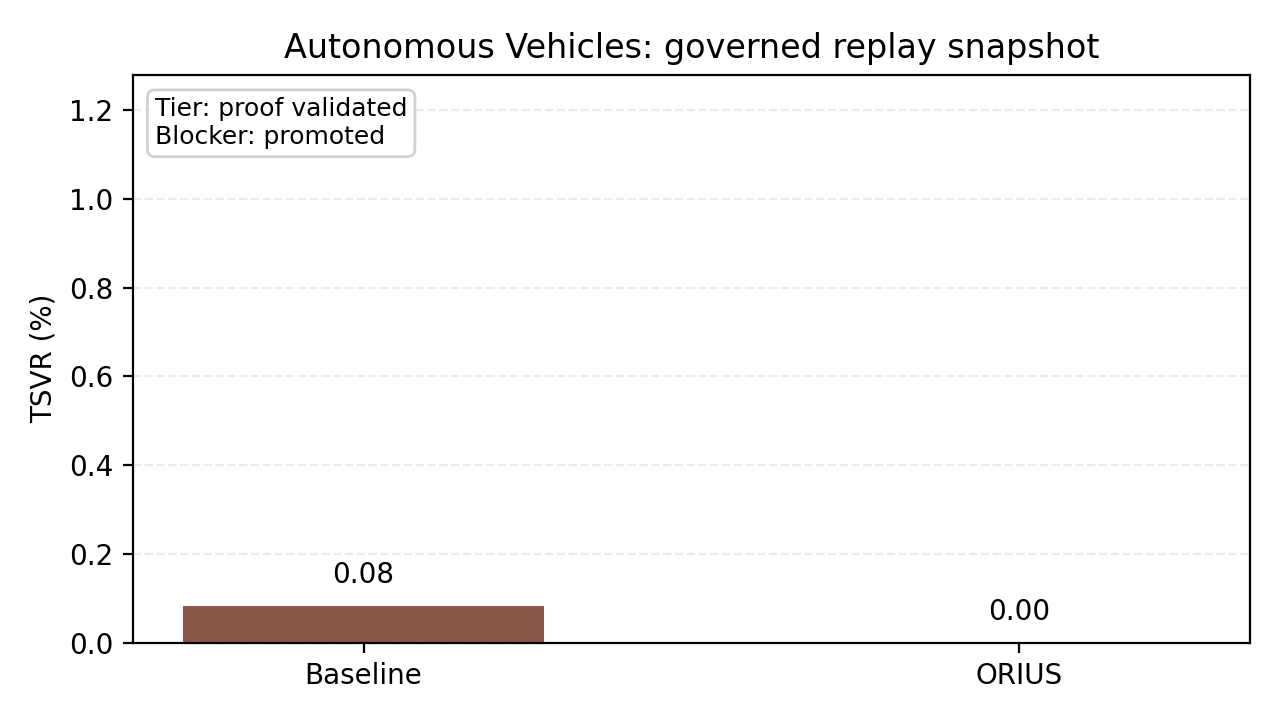
\includegraphics[width=0.90\textwidth]{reports/publication/fig_av_chapter_snapshot.png}%
}{%
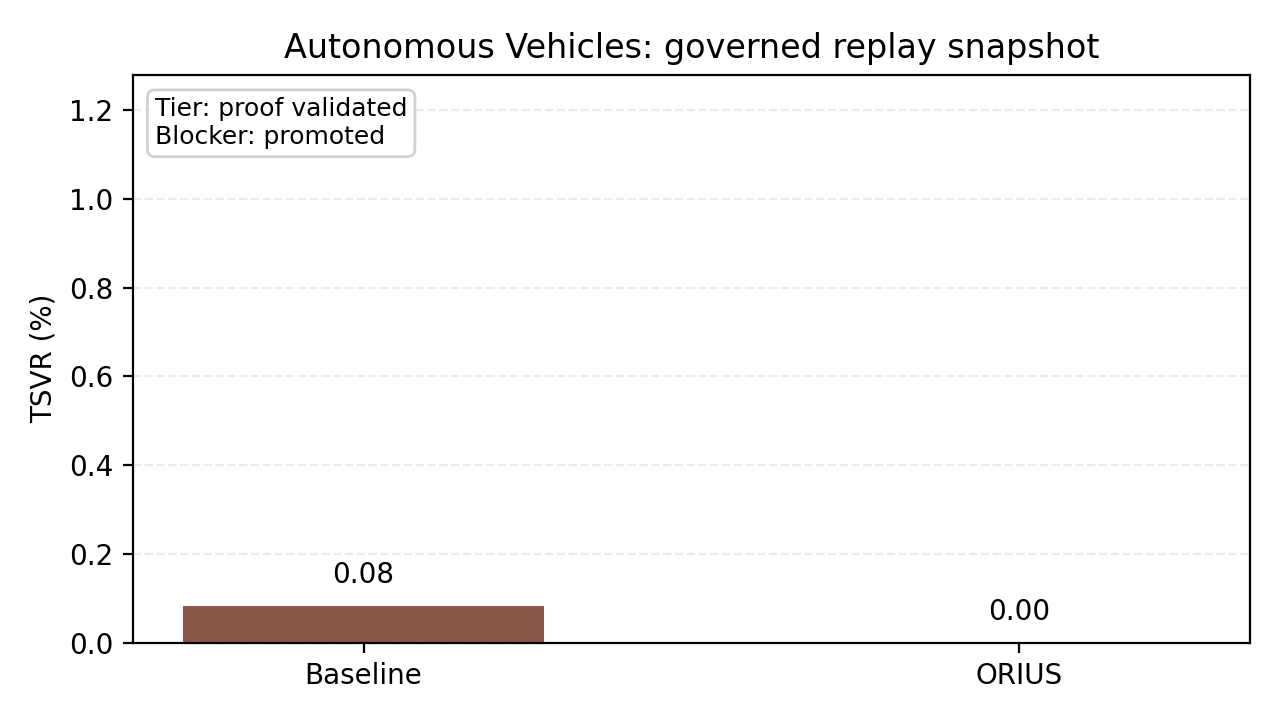
\includegraphics[width=0.90\textwidth]{../reports/publication/fig_av_chapter_snapshot.png}%
}
\caption{Autonomous Vehicles replay snapshot derived from the governed domain-closure artifact. Baseline and repaired TSVR are taken from the locked closure matrix; tier and blocker language remain governed by the parity gate.}
\label{fig:av-chapter-snapshot}
\end{figure}

\section{{Fallback and runtime behavior}}
The vehicle row uses bounded braking and TTC-aware entry gating so the runtime can refuse unsafe accelerations when the observed stopping geometry is no longer trustworthy.

\section{{Evidence tier and promotion blocker}}
The governing replay artifact for this row is the closure surface 0.0833 to 0.0000 TSVR transition under a replay status of pass. The evidence tier stays bounded by the parity gate rather than by narrative preference.



\section{{Limitations and exact non-claims}}
The row is still bounded to the current longitudinal autonomy contract. Multi-lane interaction, richer state repair, and broader deployment semantics remain outside the present validated surface. This row does not claim full-stack autonomous-driving safety or equal closure for multi-agent highway interaction; it claims bounded longitudinal closure under the current TTC contract.

The current promotion obligation for this row remains explicit: Future promotion work must preserve the single-contract TTC semantics, replay-backed soundness checks, and explicit fallback compatibility instead of reopening multiple competing repair formulations.
